% leukemia problem

\documentclass[a4paper]{article}
\usepackage{graphicx}
\usepackage{amsmath}
\usepackage{color}

\begin{document}
\section{Optimal control of leukemic cell populations}
We study the optimal control of leukemic cell population presented in \cite{Dupuis14}, namely the optimal use of a combination of 
cytostatic and cytotoxic drugs in order to reduce the total cancerous cells.
The model from \cite{Adimy08,Mackey78} considers two sub-populations of leukemic cells: the inactive resting cells, and the proliferating cells.
Resting cells  go into the proliferating phase at constant rate $\beta$.
Proliferating cells either die by apoptosis with rate $\gamma$ or divide during mitosis into two daughter cells.
Mitosis has a duration of $2 \tau$ and the daughter cells start in the resting phase.
We introduce the age variable $a$ for the time spent in the proliferating phase, and note $R(t)$ the resting population and $p(a,t)$ the proliferating population.
We consider two drugs: a cytotoxic that induces a death rate $u(t)$ in the second half of the proliferating phase, and a cytostatic $v$ that results in a fraction
$k(t)$ of inhibited resting cells that are blocked from entering the proliferating phase.
This age-structured model is represented on Fig. \ref{fig:hematoModel}.
\begin{figure}[h!]
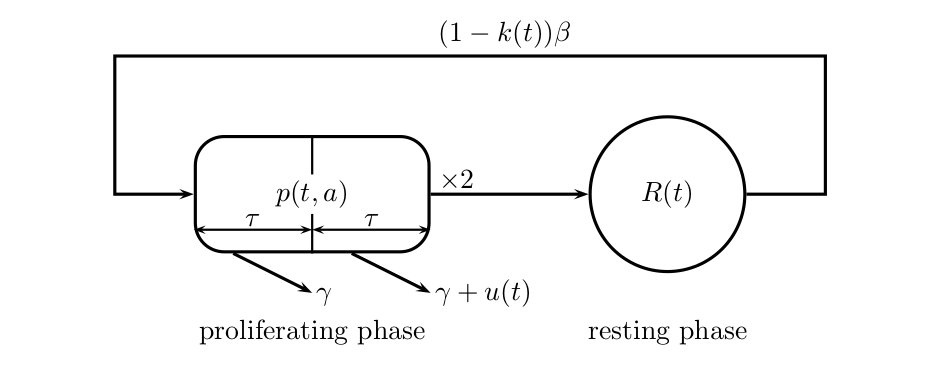
\includegraphics{hematoModel}
\caption{\label{fig:hematoModel} Age-structured model}
\end{figure}

\noindent The system follows the dynamics
$$
\begin{array}{l}
\frac{dR}{dt}(t) = -(1-k(t)) \beta R(t) + 2p(t,2\tau)\\
\frac{dk}{dt}(t) = v(t) (1-k(t)) - \alpha k(t)\\
\frac{\partial p}{\partial t}(t,a) + \frac{\partial p}{\partial a}(t,a) = -(\gamma + \chi_{(\tau,2\tau)}(a)u(t)) p(t,a) \quad 0<a<2\tau\\
p(t,0) = (1-k(t)) \beta R(t)
\end{array}
$$
In order to handle the transport equation for $p$, we note the total and second half proliferating populations
$$
P(t) = \int_0^{2\tau} p(t,a)da, \quad P_2(t) = \int_\tau^{2\tau} p(t,a)da
$$
As detailed in \cite{Dupuis14,Adimy08}, by the method of characteristics the dynamics can be rewritten as a system of delay differential equations 
corresponding to a controlled version of Mackey's model \cite{Mackey78}.
$$
\begin{array}{ll}
\frac{dR}{dt}(t) = & -(1-k(t)) \beta R(t) + 2(1-k(t-2\tau)\beta R(t-2\tau)e^{-(\gamma 2 \tau + \int_{t-\tau}^\tau u(s) ds)}\\
\frac{dP}{dt}(t) = & -(\gamma P(t) + u(t)P_2(t)) + (1-k(t))\beta R(t) \\ 
& - (1-k(t-2\tau))\beta R(t-2\tau) e^{-(\gamma 2 \tau + \int_{t-\tau}^\tau u(s) ds)}\\
\frac{dP_2}{dt}(t) = & -(\gamma + u(t)P_2(t)) + (1-k(t-\tau))\beta R(t-\tau)e^{-\gamma \tau}\\
& - (1-k(t-2\tau))\beta R(t-2\tau) e^{-(\gamma 2 \tau + \int_{t-\tau}^\tau u(s) ds)}\\
\frac{dk}{dt}(t) = & v(t) (1-k(t)) - \alpha k(t)
\end{array}
$$

We refer the reader to \cite{Dupuis14} for the formal analysis of this system, namely the existence of solutions and the 
introduction of age-weighted populations $\tilde{P}, \tilde{P_2}$ to counteract the horizon effect that would cause 
to always stop all treatment at the end of the time interval.
Taking into account constraints on the maximal cumulative dose of drugs, the resulting optimal control problem writes as
$$
\left \lbrace \begin{array}{l}
Min \ R(T) + \tilde{P}(T)\\
\frac{dR}{dt}(t) = -(1-k(t)) \beta R(t) + \tilde{p}(t,2\tau)\\
\frac{d\tilde{P}}{dt}(t) = \lambda \tilde{P}(t) - u(t) \tilde{P}_2(t) + \tilde{p}(t,0) - \tilde{p}(t,2\tau)\\
\frac{d\tilde{P}_2}{dt}(t) = (\lambda - u(t)) \tilde{P}_2(t) + \tilde{p}(t,\tau) - \tilde{p}(t,2\tau)\\
\frac{dk}{dt}(t) = v(t) (1-k(t)) - \alpha k(t)\\
0 \le u(t) \le \bar{u}, \quad 0 \le v(t) \le \bar{v}\\
\int_0^T u(t) dt \le \bar{U}
\end{array} \right .
$$
where $\lambda$ is defined by the equation $\lambda+\beta = 2 \beta e^{-(\lambda+\gamma)2\tau}$ and
$$
\begin{array}{l}
\tilde{p}(t,0)  =  (1-k(t))(\lambda+\beta)R(t)\\
\tilde{p}(t,\tau)  =  (1-k(t-\tau))(\lambda+\beta)R(t-\tau)e^{\lambda \tau}\\
\tilde{p}(t,2\tau)  =  (1-k(t-2\tau))(\lambda+\beta)R(t-2\tau)e^{\lambda 2\tau - y(t)}\\
y(t)  = \int_{t-\tau}^t u(s)ds
\end{array}
$$
with the border cases
$$
\begin{array}{ll}
\tilde{p}(t,\tau)  = p_0(\tau-t)2 e^{-\gamma t - (\lambda+\gamma)\tau} &\quad \text{if } t<\tau\\
\tilde{p}(t,2\tau)  = p_0(2\tau-t)2 e^{-\gamma t - y(t)} &\quad \text{if } t<2\tau \\
y(t)  = \int_0^t u(s)ds &\quad \text{if } t<\tau\\
\end{array}
$$

\noindent From \cite{Dupuis14} we take the initial conditions
$$
R(0)=R_0 = 4\ 10^5,\ k(0)=0,\ y(0)=0,
$$
$$
\tilde{P}(0)=\int_0^{2\tau}e^{(\lambda+\gamma)(a-2\tau)}p_0(a)da, \quad \tilde{P}_2(0)=\int_\tau^{2\tau}e^{(\lambda+\gamma)(a-2\tau)}p_0(a)da.
$$
and the parameters
$$
T=5,\ \tau=1,\ p_0(a)=0.5\ 10^5,\ \alpha=1,\ \beta=2,\ \bar{v}=2,\ \gamma=0.05.
$$

\noindent Numerical simulations are carried out for three cases: $\bar{u}=0.2$, $\bar{U}=2\bar{u}$ (Fig. \ref{fig:fig3});
$\bar{u}=1$, no limit $\bar{U}$ (Fig. \ref{fig:fig4}); and $\bar{u}=1$, $\bar{U}=2\bar{u}$ (Fig. \ref{fig:fig5}).

\begin{figure}[h!]
 \begin{center}
  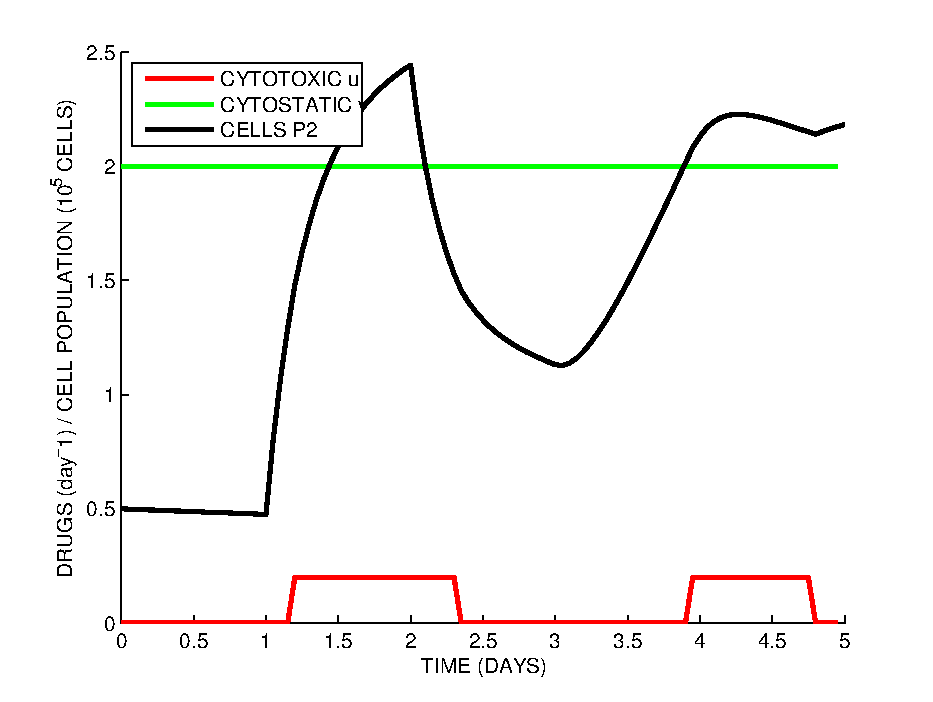
\includegraphics[width=0.5\textwidth]{Fig3}
  \caption{\label{fig:fig3} Low cytotoxic dose $\bar{u}=0.2$, with cumulative limit. Optimal solution is bang-bang with cytotoxic administered when sub-population $P_2$ is high.}
  \end{center}
\end{figure}

\begin{figure}[h!]
 \begin{center}
  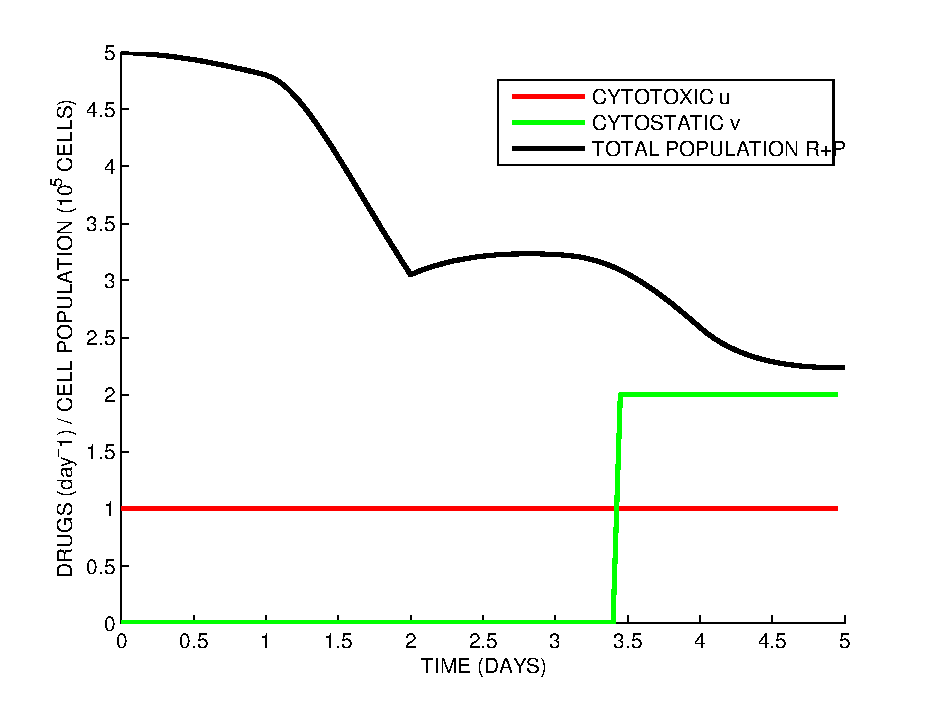
\includegraphics[width=0.5\textwidth]{Fig4}
  \caption{\label{fig:fig4} High cytotoxic dose $\bar{u}=1$, without cumulative limit. Optimal cytostatic is bang-bang.}
  \end{center}
\end{figure}

\begin{figure}[h!]
 \begin{center}
  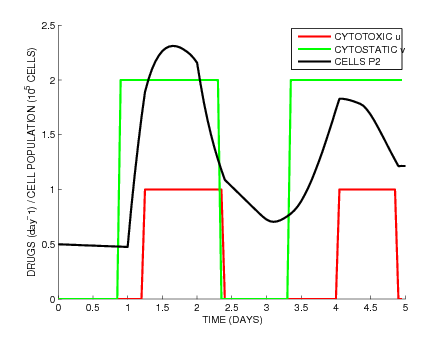
\includegraphics[width=0.5\textwidth]{Fig5}
  \caption{\label{fig:fig5} High cytotoxic dose $\bar{u}=1$, with cumulative limit. Both optimal cytostatic and cytotoxic are bang-bang.}
  \end{center}
\end{figure}

\bibliographystyle{plain}
\bibliography{leukemia}

\end{document}